\documentclass[11pt,a4paper]{ivoa} 
\input tthdefs

\usepackage{makecell}
\usepackage{listings}
\usepackage[normalem]{ulem}
\usepackage{fancyvrb}
\usepackage{appendix}
\usepackage{amsmath}
\lstloadlanguages{C}
\lstset{flexiblecolumns=true,numberstyle=\small,showstringspaces=False,
  basicstyle=\ttfamily,defaultdialect=[latex]tex,language=tex}

\usepackage[colorinlistoftodos]{todonotes}

\usepackage[utf8]{inputenc}

\usepackage{titlesec}
\titleformat{\paragraph}
{\normalfont\normalsize\bfseries}{\theparagraph}{1em}{}
\titlespacing*{\paragraph}
{0pt}{3.25ex plus 1ex minus .2ex}{1.5ex plus .2ex}


\definecolor{texcolor}{rgb}{0.4,0.1,0.1}
\newcommand{\texword}[1]{\texttt{\color{texcolor} #1}}

\iftth
  \newcommand{\BibTeX}{BibTeX}
\fi
\newcommand\apj{The Astrophysical Journal}
\newcommand\jcap{Journal of Cosmology and Astroparticle Physics}
\newcommand\prd{Physical Review D}
\newcommand\aap{Astronomy \& Astrophysics }

\iftth
 \newcommand{\comicstuff}[1]{
    \begin{html}<span class="comic">#1</span>\end{html}}
\else
  \newcommand{\comicstuff}[1]{(HTML exclusive material)}
\fi
\customcss{custom.css}

\newcommand\ada[1]{\textcolor{red}{\textbf{#1}}}
\newcommand\daniel[1]{\textcolor{blue}{\textbf{#1}}}
\newcommand\pierre[1]{\textcolor{orange}{\textbf{#1}}}
\newcommand\fxp[1]{\textcolor{teal}{\textbf{#1}}}
%% Switch the comment between the following lines to see/hide previous versions of the text
%%\newcommand\add[1]{\fxp{#1}}
%%\newcommand\remove[1]{\xout{#1}}
%%\newcommand\replace[2]{\remove{#1} \add{#2}}
%\newcommand\add[1]{#1}
%\newcommand\remove[1]{}
%\newcommand\replace[2]{\add{#2}}


\title{MOC: Multi-Order Coverage map}

\ivoagroup{Applications}

\author{Francois-Xavier Pineau (CDS)}
\author{Pierre Fernique (CDS)}
\author{Ada Nebot (CDS)}
\author{Daniel Durand (CADC)}
\author{Matthieu Baumann (CDS)}
\author{Thomas Boch (CDS)}
\author{Baptiste Cecconi (LESIA, Observatoire de Meudon)}
\author{Giuseppe Greco (EGO-Virgo)}
\author{Tom Donaldson (STScI/NASA)}
\author{Thomas Robitaille}
\author{Mark Taylor (University of Bristol)}
\author{Wil O'Mullane (Vera C. Rubin Observatory)}
\author{Martin Reinecke (Max Planck)}
\author{S\'{e}bastien Derri\`{e}re (CDS)}

\editor{Francois-Xavier Pineau}
\editor{Pierre Fernique}
\editor{Ada Nebot}
\editor{Daniel Durand}

\previousversion[http://ivoa.net/documents/MOC/20220727]{Version2.0}
\previousversion[http://ivoa.net/documents/MOC/20191007]{Version1.1}
\previousversion[http://ivoa.net/documents/MOC/20140602]{Version1.0}

\begin{document}

\begin{abstract}
This document defines version 2.1 of the Multi-Order Coverage map (MOC) method,
which enables the specification of arbitrary coverages across sky regions,
time intervals and frequency domains.

The goal is to be able to
provide a very fast comparison mechanism between coverages. The
mechanism relies on discretizing the unit sphere and one-dimensional quantities
such as time or frequency.
Specifically, the discretization uses the Z-order curve for 2-dimensional sky
regions and on hierarchical dyadic subdivisions for 1-dimensional quantities.
The system is based on the definition of a specific storage
of the map coverage using predefined cells hierarchically grouped
which makes it easy to produce and use for exploring astronomical
collections.
This version 2.1 extends the use of MOCs to the three physical quantities:
space, time, frequency, as well as their pairwise combinations.
\end{abstract}

\listoffigures
\listoftables 
%\todototoc
%\listoftodos[Issues which need attention]


\section*{Acknowledgments}
This work has been supported by the ESCAPE project (the European
Science Cluster of Astronomy \& Particle Physics ESFRI Research
Infrastructures) that has received funding from the European Union's
Horizon 2020 research and innovation Programme under the Grant
Agreement n.\ 824064.

\section*{Conformance-related definitions}
The words ``MUST'', ``SHALL'', ``SHOULD'', ``MAY'', ``RECOMMENDED'',
and ``OPTIONAL'' (in upper or lower case) used in this document are to
be interpreted as described in IETF standard RFC2119
\citep{std:RFC2119}.

The \emph{Virtual Observatory (VO)} is a general term for a collection
of federated resources that can be used to conduct astronomical
research, education, and outreach.  The
\href{http://www.ivoa.net}{International Virtual Observatory Alliance
  (IVOA)} is a global collaboration of separately funded projects to
develop standards and infrastructure that enable VO applications.

\begin{figure}[!htbp]
\begin{center}
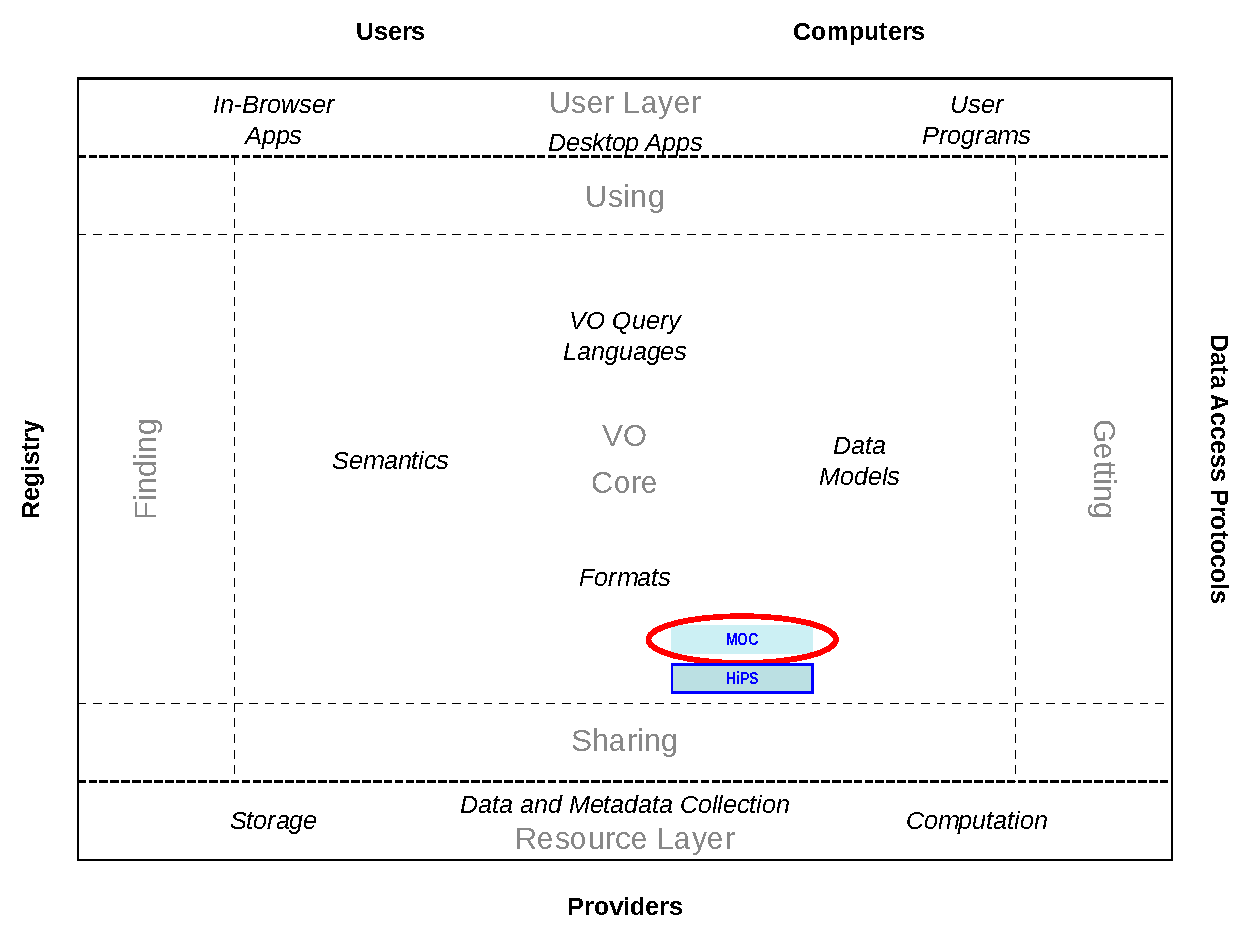
\includegraphics[width=0.9\textwidth]{role_diagram.pdf}
\end{center}
\caption[IVOA architecture diagram]{Architecture diagram for Multi-Order Coverage map.}
\label{fig:ivoadiagram}
\end{figure}

\section{Introduction}
This document is a minor release of the already existing encoding method
recommendation \emph{Multi-Order Coverage} map
\citep[MOC~2.0,][]{2022ivoa.spec.0727F}.
We generalize the MOC originally limited to Space, Time, and Space-Time
dimensions (Space MOC, SMOC; Time MOC, TMOC; and Space-Time MOC, STMOC)
to the Frequency, Space-Frequency and Frequency-Time dimensions
(Frequency MOC, FMOC; Space-Frequency, SFMOC; Frequency-Time, FTMOC).
Figure~\ref{fig:ivoadiagram} illustrates the role MOC 2.1
plays within the IVOA architecture \citep{2021ivoa.spec.1101D}.

The encoding method described in this document allows one to define
and manipulate space, time and frequency coverage in such a way that basic
operations like union, intersection or equality test can be performed
very efficiently. This methodology allows VO applications and
data servers to build efficient
procedures to perform such operations on observations and catalogs.
In the next sections we will describe the different MOCs and their
encoding standards.

\section{The rationale}
\label{sec:usecases}
The goal behind the MOC is to get a method to manipulate coverages in
order to provide very fast union, intersection and
equality operations between them. In order to accomplish this task, we
based the system on a regular and hierarchical discretization as
exposed below.
The evolution of the MOC standard -- which was initially limited to spatial
quantities in version 1.0, then expanded to include temporal quantities in
version 2.0, and finally supplemented with frequency quantities in version
2.1 -- enables it to cover a wide range of astronomical use cases, e.~g.:
\begin{itemize}
\item What are the space and time coverages of the 2MASS observations
  and are there any observations which are coincidental with the HST
  archive?
\item Which are the astronomical catalogs which have data for a list
  of Supernova events within a given time window?
\item Are there any other observations coincidental with this
  gravitational wave detection given its time and spatial coordinates?
\item Are there quasi-simultaneous observations (within a given time
  window) of these two surveys for a list of eclipsing binaries?
\item Find the intersection between the SDSS coverage and the
  ephemeris of this Near Earth Object, was it observed by SDSS? And
  by Galex? By both missions simultaneously? If so, are there
  detections within the source catalogues?
\item Has Neptune been observed by DSS?
\item Is a radio source contaminating my observations in given frequency
  ranges?
\end{itemize}

It was possible to answer those questions with MOC 1.0 standard and
other VO tools but the amount of manipulation and computation was
quite a big hurdle for the researchers. With MOC 2.0 it is possible
to answer these questions in a few milli-seconds. Another example
of usage would be the visual inspection of the spatio-temporal
coverage of PanSTARRS observations (see Figure~\ref{fig:panstarrs}).
The choice of a temporal resolution and a spatial resolution makes it
possible to obtain a MOC of a desired data volume.

\begin{figure}[!ht]
\begin{center}
\includegraphics[width=\textwidth]{panstarrs.png}
  \caption[STMOC of PanSTARRS observations]{PanSTARRS observations and the associated spatial and
  temporal coverage within three different periods of time.
  The volume of the PanSTARRS MOC at a temporal resolution
  of about 17 minutes and spatial resolution of 52 arcsec is 320\,MB.}
\label{fig:panstarrs}
\end{center}
\end{figure}

\subsection{Comparing the coverage of multiple data sets}
The computation of data set intersections using the MOCs is simple (it
is simply a list comparison). The result of any operation is itself a
MOC which can be used in further operations. For instance it is
possible to compute the intersection of Saturn's ephemeris and
the spatio-temporal coverage of HST ACS observations, and subsequently,
query a database for retrieving images for which time and position
fall within this intersection (see Fig.~\ref{fig:stmoc-saturn}).

\begin{figure}[h]
\begin{center}
\includegraphics[width=\textwidth]{stmoc_op.png}
\end{center}
\caption[Intersection of HST ACS and Saturn STMOCs]{Intersection of HST ACS observations
      and Saturn ephemeris Space-Time-MOC}
\label{fig:stmoc-saturn}
\end{figure}

\subsection{Query databases using MOC}
In principle, querying a positional database using complex sky region
coverage is possible using ADQL. However, this is rarely possible
when the sky region has to be described as unions and intersections of
sub-regions to cover a complex, non regular area. In practice, most
existing ADQL implementations only support simple regions
(cones, boxes, polygons), and can rarely deal with unions and
intersections unless by joining independent queries – and this even if
the described region is, in fact, empty!  If databases are adapted to
supporting MOC based queries, they will offer then a useful method
allowing any kind of sky region query. In addition, if the internal
spatial index of the database is itself based on HEALPix, the
filtering will then be straightforward and all the intermediate sky
computations will be removed providing an optimal response time.

\subsection{Gravitational Wave localisations}
The contours of a gravitational-wave sky localization are constructed
as follows. The pixels from most probable to least are ranked, and summed
up to get a fixed level of probability \citep{2014ApJ...795..105S}.
In practice, the HEALPix pixels inside a given contour plot are extracted,
and the MOC coverage is generated from the table made up from the pixels.
Every single level of probability can be used as a regular MOC even in the case in
which the sky localization is irregularly shaped with disjoint regions.
This coding technique allows for an extra fast integration in the existing
Virtual Observatory structures and
tools\footnote{\url{https://emfollow.docs.ligo.org/userguide/}}.
The 2D contours of a GW sky localization can be visualised
and manipulated using Aladin Desktop, allowing one to compare them with
existing surveys, overlap sky map generations with increasing accuracy
and computational cost and query the VizieR database.
These sets of tasks can also be performed via Python using the astropy
affiliated package mocpy\footnote{\url{https://cds-astro.github.io/mocpy/}},
efficiently displayed in javascript applications
with Aladin Lite, and integrated within Jupyter notebooks through the
ipyaladin\footnote{\url{https://cds-astro.github.io/ipyaladin/}}
widget\footnote{\url{https://pos.sissa.it/357/031/pdf}}.


\subsection{Space and Time MOC: Einstein Telescope and Early Warning Alerts}
The space and time MOC provides us with an effective way to develop new
multi-messenger data analysis tools that will have a crucial role when
the third-generation interferometric gravitational wave observatories,
such as the Einstein Telescope (ET), will begin operation. Here we
figure out a few potential applications. ET will explore the universe
with gravitational waves up to cosmological distances with an
expected detection rate of order $10^{5} - 10^{6}$ black holes and $7\times10^4$
neutron star mergers per year \citep{2020JCAP...03..050M}.
For fast and real time data access, the user can query by a specific
time range the gravitational-wave sky localizations encoded as a space
and time MOC.

In addition, the ET sensitivity at low frequencies enables enough
signal-to-noise ratio to accumulate before the merger, making possible
a pre-merger gravitational-wave detection and warning for the
electromagnetic/neutrino follow up.  The simulations show that, by
requiring a signal-to-noise ratio $>=$ 12 and a sky localization smaller
than 100 deg$^2$, ET can send an early warning alert between 1 and 20 hours
before the merger (with the mean of the distribution at about 5 hours)
for signals at 40 Mpc \citep{2018PhRvD..97l3014C}. The
electromagnetic/neutrino survey can benefit
in multiple spatial and temporal intersections with a gravitational-wave
sky localization to probe any electromagnetic/neutrino signals temporally
and spatially connected to the inspiral, merger or ring-down phases.
Early warning alerts are also planned in the LIGO-Virgo-KAGRA O4 run with
an experimental capability to produce and distribute early warning
gravitational-wave alerts up to tens of seconds before
merger\footnote{\url{https://emfollow.docs.ligo.org/userguide/early_warning.html}}.

\subsection{Multi-site search in space, time and/or frequency}
Often, a typical query from a virtual observatory (VO) user is to
request all possible records from the VO at a given sky position
and/or at a given time, and/or at a given frequency.
While this is in principle possible by dispatching one narrow positional
query to every registered Cone Search, SSA or SIA service and filtering
by time, in practice, the number of queries required leads to an unacceptable
load on both clients and services. Moreover, most of these queries will
deliver no results since most services often lack coverage in the queried
region. If basic footprint/coverage information was available for all
registered services, for instance using VODataService 1.2
\citep{2021ivoa.spec.1102D} only those with coverage in the region
and time/frequency of interest would then be queried. This would provide a
great reduction in the number of services to be queried optimizing the
response time. Using the MOC offers the opportunity to provide this
coverage information in a uniform way. The MOC could be stored locally
for a given service or centrally where the coverage for a number of
services would be supported.

\subsection{Low frequency radio astronomy}

Ground-based low-frequency radio astronomy instruments typically span over
a wide spectral range, such as from 10 MHz to 85 MHz, with NenuFAR
\citep{zarka_2028}, which covers a factor of 8.5 in spectral domain.
The main beam of the instrument has a field of view that varies by almost one
order of magnitude. Due to its interferometric nature, the shape of the side
lobes varies in frequency.
Astronomers preparing observations with NenuFAR need to identify and assess
any contaminating radio sources that may be visible in the side lobes of
the instrument.
The current NenuFAR Python library \citep[nenupy,][]{loh_2025} implements this
assessment by cross-matching a series of spatial MOCs (for the grating lobes
and the interfering bright radio sources) with a temporal and spectral sampling.
Merging the spatial and spectral dimensions into an spatio-frequency MOC
for a series of observation times would simplify and speed up this task.

The low-frequency radio sources observed in our solar system,
such as the Sun or the magnetised planets, but also those of active stars
and some exoplanetary systems, are showing very dynamical structures in the
temporal-spectral domain, at time scales spanning from milliseconds to hours.
The TFCat \citep[Time-Frequency catalogue,][]{cecconi_2023} has been developed
to represent observed features in the temporal-spectral domain, using, e.g.,
polygons in physical coordinates.
While this framework proved to be very efficient to store, share, and display
those features, cross-matching the catalogues is still a difficult process.
Transforming each of the catalogues into an frequency-time MOC would
allow very efficient identification of possibly simultaneous events listed
in different catalogues.


\section{MOC principles}

Irrespective of the quantity, the MOC standard is defined using four basic
building blocks: discretization, unique reference system, hierarchization
and efficient encoding:
\begin{enumerate}
\item Determine a proper tessellation/discretization methodology for
  each quantity (space, time, frequency, ...);
\item Fix a unique referential system for each quantity, to avoid
  reference conversions and thus allowing to easily compare different
  data collections;
\item Use an hierarchical procedure and a unique representation
  (canonical form) for compacting and quickly manipulating
  coverages of a given quantity at any level of accuracy;
\item Implement at least one serialization in a binary encoding format
  (other serializations are possible, e.g. ASCII).
\end{enumerate}

With these principles, a MOC consists of a list of numbers which
represent the indices of the cells mapping the coverage of the spatial,
temporal or frequency axis.
As soon as the consecutive cells are used at order n, they will be
hierarchically grouped in their parent cell at order n-1, and
this recursively. This introduces the notion of orders and
associated cell index boundary alignment implied by the hierarchical structure
facilitates the combination of cells at different orders.

\medskip
\par\noindent
We will now explain the conventions chosen for single quantity MOCs,
namely space, time and frequency MOCs designated by the acronyms SMOC,
TMOC and FMOC.
Then, we also explain the conventions chosen for two-dimensional MOCs,
namely space-time, space-frequency and frequency-time MOCs
designated by the acronyms STMOC, SFMOC and FTMOC.

\subsection{Single quantity MOCs}

In this section, we describe the convention relative to single quantity MOCs.

\subsubsection{Space MOC conventions}
Defining a sky region by a subset of regular sky tessellation or tiles
is not a new idea.  In astronomy, one could find three main methods of
partitioning the sphere : Q3C, HTM and HEALPix which are respectively
using cells in the form of squares, triangles and diamonds for mapping
the celestial sphere.

Several publications have compared these methods \citep{2001misk.conf..638O}. We
justified the choice of HEALPix for the MOC because of these four
points:

\begin{itemize}
\item Equal areas: by construction, HEALPix consists of diamond cells with
  equal spherical surfaces. Thus the area of a given region is trivial
  to compute;
\item Computing time: HEALPix has the peculiarity that the computing
  time does not depend on the hierarchical order \footnote{Note that in the HEALPix
  document orders are refered to as levels, and cells as diamonds.}
  (no recursive  algorithm);
\item Accuracy: HEALPix provides libraries which allow the calculation
  up to accuracy of 0.4 mas (order 29) (\url{http://sourceforge.net/projects/healpix/});
\item Standard: Existence of many HEALPix libraries: C++, Java,
  Fortran, Python, Rust, Web Assembly, ...
  Also, HEALPix was selected for several all sky
  missions such as WMAP, Planck and Gaia. The HEALPix main web site, previsously
  located at Jet Propulsion Laboratory, is now on sourceforge (\url{http://healpix.sourceforge.io/}).
\end{itemize}

The HEALPix \citep{2005ApJ...622..759G} NESTED tessellation technique divides
the sphere into 12 cells, each of them sub-divided into 4 cells
recursively (see Fig.~\ref{fig:healpix}). Thus the sphere at order 1
will consist of 48 cells,
192 cells at order 2, 768 at order 3 and so on where each cell
at a given order is covering an equal area of the sphere.

\begin{figure}[!htbp]
\begin{center}
\includegraphics[scale=0.8]{healpix.jpg}
\end{center}
\caption{HEALPix partition of the sphere}
\label{fig:healpix}
\end{figure}


In practice, the sub-division of each base cell -- which are squares in the
Euclidean HEALPix projection plane -- consists in iterations of a Z-order
curve, and bit interleaving allows for a non-recursive algorithm.
When encoding a "NESTED" HEALPix index, the four Most Significant Bits (MSB) are used to code
the base cell index ($ \in [0, 12[)$ and the remaining LSBs are the 2-dimensional Morton code of the
coordinates inside the base cell.

Thus, the "NESTED" numbering consists of enumerating all cells in a
specific order. For instance, at order 1, there are 48 cells (12x4)
enumerated from 0 to 47. In this scheme, the 4 sub-cells of cell M
have the indices: (M$\times4)+3$, (M$\times4)+1$, (M$\times4)+2$,
(M$\times4$) in reading
order. And reciprocally, the parent index of cell N is
N/4. Each SMOC cell is coded by a pair of numbers:
(order, index) which are the HEALPix order and the HEALPix index in this
order.

\begin{figure}[h]
\begin{center}
\includegraphics[width=\textwidth]{nested_healpix.jpg}
\end{center}
\caption{HEALPix numbering principle}
\end{figure}

To support the encoding based on 64-bit longs, the best resolution
available is provided at order 29 and according to the HEALPix
equations, corresponds approximately to 0.4mas.  The SMOC resolution
is set by the maximum value of the HEALPix order used to define a
region. Its selection depends on the accuracy chosen by the provider
to define the region. As data set boundaries are not aligned with the
HEALPix cell borders, a SMOC is generally an upper-approximation of
the data set coverage. The quality of this approximation depends
directly on the chosen SMOC resolution (MOCORD\_S).
Table~\ref{table:orders} provides the HEALPix cell angular resolution for
each HEALPix order.

In Figure~\ref{fig:smoc-view} we show the MOC creation, from images to their coverage,
and indicating their corresponding HEALPix numbers.

\begin{figure}[h]
\begin{center}
\includegraphics[width=\textwidth]{smoc_view.png}
\end{center}
\caption[SMOC from an image]{SMOC: from the image
      to the list of numbers based on HEALPix hierarchy tessellation}
\label{fig:smoc-view}
\end{figure}

\input{table1.tex}
\input{table2.tex}

The formula computing a cell index from a sky location is described in
the main article defining the HEALPix system \citep{2005ApJ...622..759G}.
Several support libraries implementing the most
important primitives are already available. These libraries are required
for generating SMOCs and for comparing them with sky coordinates.
However, they do not provide built-in support for performing basic
SMOC arithmetic operations.



\subsubsection{Time MOC conventions}
\label{sec:tmoc1}


In order to represent time coverage, we need to select a-priori the
total range of time that we will cover with the notation. Following
the same SMOC principles, we need to use a discrete time axis where
each unit element of this axis has a constant duration. We adopt
the Julian Date convention, very common in astronomy and a nominal
resolution of 1$\mu$s. The temporal dimension being by nature 1D unlike
the spatial dimension, we opt for a order progression by factor of
2 (4 for SMOC) and therefore 62 orders (30 for SMOC). This way we
can address $2^{62}$ cells in an unsigned 64-bit integer,
i.e. a little bit more than 73000 years at
1$\mu$s resolution, enough for most astronomical time events. At the
deepest order (61) the TMOC cell number is the number of $\mu$s since
JD=0.
Hence, ab integer time value $t$ in $\mu$s since JD=0 is valid if
$t \in [0, 2^{62}[$. For a given $order$, its cell $index$ is:
\begin{equation}
  index = \frac{t}{2^{order}}
  \label{eq:tmoc:i}
\end{equation}
Conversly, the range of time values $[t_{min}, t_{max}[$, in $\mu$s since JD=0,
of a given $index$ of order $order$ is given by
\begin{align}
  t_{min} &= index \times 2^{order} \\
  t_{max} &= (index + 1) \times 2^{order}
  \label{eq:tmoc:t}
\end{align}.

We note that two consecutive cells at order N with the indices
(M$\times$2)+1, (M$\times$2) will be coded at order N-1 with the index
M and thus recursively. The order N-1 cell duration is 2 times more
than the N cell duration (61: 1 $\mu$s, 60: 2 $\mu$s, 59: 4 $\mu$s, etc...).

The time is a relative observation, and depends on the position of the
observer. There are many time scales for measuring time:
Terrestrial Time (TT), Barycentric Coordinate Time (TCB), Geocentric
Coordinate Time (TCG), Ephemeris Time (ET), Barycentric Dynamic Time
(TDB), International Atomic Time (AI), etc. We opt for the TCB
reference (see \cite{2015A&A...574A..36R} for details).

TMOC {\bf must} be based on the time scale TCB (see section~\ref{sec:tcb})
and the Solar System Barycenter as the reference position
\citep[see also][]{2019ASPC..523..497F} and section~\ref{sec:tmoc1}.

It may be necessary to convert the temporal events to the
chosen scale. If the ephemeris required for this conversion are
not available, opt to degrade the accuracy of the time measurement
(typically around 20 minutes for observations within the Earth orbit
environment to cover all possible observer positions).
Table~\ref{table:tmocorders} shows the time resolutions of the cells
for each possible order.

In Figure~\ref{fig:tmoc-view} we show the creation of TMOC, from a time
series to the list of numbers based on time discretization.
 
\begin{figure}[h!]
\begin{center}
\includegraphics[width=\textwidth]{tmoc_view.png}
\end{center}
\caption[TMOC from time series]{TMOC: from the
      time series to the list of numbers based on time
      discretization}
\label{fig:tmoc-view}
\end{figure}

\subsubsection{Frequency MOC conventions\label{sec:fmoc1}}

As for Time, representing a frequency coverage requires defining \emph{a priori}
the total frequency range to be described by the notation. However, unlike Time --
which is expressed as milliseconds since a reference epoch and therefore has a constant
absolute resolution (1 millisecond) -- frequency values are represented as floating-point
numbers with an approximately constant \emph{relative} resolution (i.e. a fixed number of significant digits),
rather than a constant absolute resolution.

The adopted\footnote{To handle floating-point quantities, two approaches have been proposed.
The first implemented solution is described in Appendix~\ref{sec:apx:fmoc1}.
It was later replaced by the more WCS-compliant solution presented above.} approach is fully generic.
First, we define the global valid frequency range $[f_{min}, f_{max}[$.
The frequency $f$ {\bf must} be expressed in $Hz$.
Next, we introduce a bijective mapping
\[
g: [f_{min}, f_{max}[ \rightarrow [0,1[
\]
such that any frequency $f \in [f_{min}, f_{max}[$ is associated with the dyadic interval containing $g(f)$.

For a given $order$, the interval $[0,1[$ is subdivided into $2^{order+1}$ dyadic intervals (the MOC cells),
indexed from $0$ to $2^{order+1}-1$.
The index corresponding to a frequency $f$ at order $order$ is therefore:

\begin{equation}
  index = \lfloor g(f) \times 2^{order+1} \rfloor
  \label{eq:fmoc:i}
\end{equation}

The adopted bounds of the valid frequency range are:
\begin{itemize}
  \item $f_{min} = 10^{-18}$ Hz, corresponding approximately to the inverse of the age of the Universe.
  \item $f_{max} = 10^{+38}$ Hz, a somewhat arbitrary upper limit chosen so that the full range spans 56 decades in logarithmic scale.
\end{itemize}

The mapping function $g$ is defined as a linear interpolation in logarithmic space:
\begin{equation}
  g(f) = \frac{\log_{10}(f) - \log_{10}(f_{min})}{\log_{10}(f_{max}) - \log_{10}(f_{min})}
  \label{eq:fmoc:g}
\end{equation}

Combining Eq.~(\ref{eq:fmoc:i}) and Eq.~(\ref{eq:fmoc:g}) with the selected frequency range,
we obtain, for a given $order$:
\begin{equation}
  index = \left\lfloor
  \frac{\log_{10}(f) + 18}{56} \times 2^{order+1}
  \right\rfloor
\end{equation}

The number of consecutive integers that can be exactly represented by an
IEEE~754 floating-point is limited by the number of bits in the mantissa.
For double-precision floating-points, this number is 52.

Notably, for a fixed exponent, the fractional part of a floating-point number
corresponds to a dyadic rational. Consequently, there is no benefit in defining
a MOC $order$ with more cells than the number of dyadic rationals representable
with 52 bits.
Beyond this limit, the cells would be smaller than the intrinsic precision of
double-precision floating-point numbers.

For this reason, the maximum order is limited to 52 levels, ranging from 0 to
$order_{max} = 51$.
At the maximum resolution, the index corresponding to a frequency $f$ is
therefore computed as:
\begin{align}
  order_{max} &= 51 \\
  index_{51}  &= \left\lfloor
  \frac{\log_{10}(f) + 18}{56} \times 2^{52}
  \right\rfloor
\end{align}

Conversely, the frequency range $[f_{min}, f_{max}[$ corresponding to a given
index $index$ at a given order $order$ can be obtained using the inverse
transformation:
\begin{eqnarray*}
  f_{min}       & = & g^{-1}(\frac{index}{2^{order + 1}})     = 10^{ 56 \times \frac{index}{2^{order + 1}} - 18} \\
  f_{max}       & = & g^{-1}(\frac{index + 1}{2^{order + 1}}) = 10^{ 56 \times \frac{index + 1}{2^{order + 1}} - 18}	
\end{eqnarray*}

Choosing a given order is equivalent to selecting the number of mantissa bits
used to represent the mapped value in the interval $\in [0, 1[$.
In practice, this corresponds to choosing a level of numerical precision,
analogous to selecting a number of significant bits (or digits), noting that
approximately one decimal digit of precision is lost for every 3 to 4 mantissa
bits removed.
The approximate number of significant decimal digits corresponding to a given
order can be estimated using the following relation:
\begin{equation}
  n = \frac{(order + 1)}{\log_2(10)}
\end{equation}
This expression follows from the conversion between binary and decimal precision,
since one decimal digit corresponds to approximately $\log_2(10) \approx 3.32$ bits.
For example, a frequency stored using a 32-bit floating-point number provides about
24 bits of significand precision, corresponding to approximately 7 decimal digits.
To obtain a comparable precision in the hierarchical representation, an order of 29 can be chosen.
Additional values are provided in Table~\ref{table:fmocorders}.

We can also express, for a given order $order$ the relative size of cell using $g^{-1}$:
\begin{equation}
    \frac{\Delta f}{f} = \frac{g^{-1}(\frac{index + 1}{2^{order + 1}}) - g^{-1}(\frac{index}{2^{order + 1}})}{g^{-1}(\frac{index}{2^{order + 1}})} = 10^\frac{56}{2^{order + 1}} - 1
\end{equation}

\begin{table}[!htbp]
\smallskip
\begin{center}
   {\scriptsize
   \begin{tabular} {|l | l| l| l| l| l| l|}
   \hline
	   Order & Significant digits (n) & Relative size $\frac{\Delta f}{f}$ & Order & Significant digits (n) & Relative size $\frac{\Delta f}{f}$  \\
   \hline
0 & 0.3 & 1.00e28 & 26 & 8.1 & 9.61e-7 \\
1 & 0.6 & 1.00e14 & 27 & 8.4 & 4.80e-7 \\
2 & 0.9 & 1.00e7 & 28 & 8.7 & 2.40e-7 \\
3 & 1.2 & 3.16e3 & \textbf{29} & \textbf{9.0} & 1.20e-7 \\
4 & 1.5 & 5.52e1 & 30 & 9.3 & 6.00e-8 \\
5 & 1.8 & 6.50e0 & 31 & 9.6 & 3.00e-8 \\
6 & 2.1 & 1.74e0 & 32 & 9.9 & 1.50e-8 \\
7 & 2.4 & 6.55e-1 & 33 & 10.2 & 7.51e-9 \\
8 & 2.7 & 2.86e-1 & 34 & 10.5 & 3.75e-9 \\
\textbf{9} & \textbf{3.0} & 1.34e-1 & 35 & 10.8 & 1.88e-9 \\
10 & 3.3 & 6.50e-2 & 36 & 11.1 & 9.38e-10 \\
11 & 3.6 & 3.20e-2 & 37 & 11.4 & 4.69e-10 \\
12 & 3.9 & 1.59e-2 & 38 & 11.7 & 2.35e-10 \\
13 & 4.2 & 7.90e-3 & \textbf{39} & \textbf{12.0} & 1.17e-10 \\
14 & 4.5 & 3.94e-3 & 40 & 12.3 & 5.86e-11 \\
15 & 4.8 & 1.97e-3 & 41 & 12.6 & 2.93e-11 \\
16 & 5.1 & 9.84e-4 & 42 & 12.9 & 1.47e-11 \\
17 & 5.4 & 4.92e-4 & 43 & 13.2 & 7.33e-12 \\
18 & 5.7 & 2.46e-4 & 44 & 13.5 & 3.66e-12 \\
\textbf{19} & \textbf{6.0} & 1.23e-4 & 45 & 13.8 & 1.83e-12 \\
20 & 6.3 & 6.15e-5 & 46 & 14.1 & 9.16e-13 \\
21 & 6.6 & 3.07e-5 & 47 & 14.4 & 4.58e-13 \\
22 & 6.9 & 1.54e-5 & 48 & 14.8 & 2.29e-13 \\
23 & 7.2 & 7.69e-6 & 49 & 15.1 & 1.15e-13 \\
24 & 7.5 & 3.84e-6 & 50 & 15.4 & 5.73e-14 \\
25 & 7.8 & 1.92e-6 & 51 & 15.7 & 2.86e-14 \\
   \hline
   \end{tabular}
   }
\caption[FMOC order and cell resolutions in number fo significant digits]{FMOC cell resolutions in number of significant digits for each orders.}\label{table:fmocorders}
\end{center}
\end{table}



Unlike time, the finest resolution is not constant across the full frequency range.
Because frequencies are represented using 64-bit floating-point values,
the achievable precision is \textit{relative} rather than \textit{absolute}.
At the highest resolution (order 51), the relative precision is approximately $10^{-15}$,
which is close to the number of significant decimal digits provided by double-precision
floating-point numbers.

Like for time, two consecutive cells at order $N$, with indices
$(M\times 2)$ and $(M\times 2)+1$, are represented at order $N-1$
by a single cell with index $M$.
This hierarchical structure applies recursively across all orders.

Considering the dyadic structure of the intervals, a cell at order
$N-1$ spans twice the frequency range of a cell at order $N$
Consequently, the frequency resolution at order
$N-1$ is half that at order $N$.


\subsection{Two dimensional MOCs}

In this section, we describe the convention adopted\footnote{The use of
a single index obtained by interleaving the indices of two quantities,
similarly to a 2D Z-order curve, was considered but ultimately discarded.
First, the resolutions of both quantities would have been coupled, making it
impossible, for example, to describe an observational coverage with low
temporal resolution and high spatial resolution.
Second, encoding two 64-bit indices into a single 64-bit index would have
reduced the maximum achievable resolution for each quantity.}
for two-dimensional MOCs, i.e. MOCs describing the coverage of two quantities
at the same time.

To respond to the different use cases presented at the beginning of 
the document, independent single quantity MOCs are not enough.
We need to link two quantities in a global mechanism.
For example, we need to be able to select a SMOC using a time or a frequency
window.
We also need to select a TMOC or a FMOC using a spatial constraint.
Implementing this linkage would allow
the potential users to select and interact with the astronomical
collections which support space, time and/or frequency and use logical
operators between them.

Our approach combines two quantities -- time and space, frequency and space,
or time and frequency -- by associating sub-MOCs of the first quantity with
MOCs of the second quantity.
For the first quantity, the range of deepest-order indices bounding a sub-MOC
must not overlap with the one of another sub-MOC.
For the second quantity, MOCs are independent and may overlap.
In the various serializations, a 2D-MOC is represented as a set of tuples, each
consisting of a sub-MOC of the first quantity and a MOC of the second quantity.
Although the resolutions of the first and second quantities may differ, 
the resolution of each quantity remains uniform across the entire 2D-MOC.

In the remaining of the document we adopt the following convention: 
a $YX$MOC is a 2D-MOC in which $X$ is the first quantity and $Y$ the second one.


\subsubsection{Space and Time MOC conventions\label{sec:stmoc}}

In Space-Time MOCs (STMOCs), the first quantity is time and the second
quantity is space.
Consecutive time ranges associated with the same spatial coverage are
grouped into a sub-TMOC linked to their common SMOC.
The STMOC is represented as a sorted set of (sub-TMOC, SMOC) pairs.


In Figure~\ref{fig:stmoc-view} we show the visual representation of an STMOC,
in which at a given sub-TMOC we obtain the corresponding SMOC. 
 
  
\begin{figure}[h]
\begin{center}
\includegraphics[width=0.8\textwidth]{stmoc_view.png}
\end{center}
\caption[Visual representation of a STMOC]{STMOC visual representation in which
      at a given TMOC range we obtain the corresponding SMOC}
\label{fig:stmoc-view}
\end{figure}

\subsubsection{Space and Frequency MOC conventions}

In some use cases, it is desirable to combine the spatial and frequency dimensions.
Similarly to STMOCs -- see section~\ref{sec:stmoc} -- SFMOCs allow the selection of a SMOC 
within a given frequency window -- or more generally, within a FMOC.
Conversely, they can also be used to derive a FMOC subject to spatial constraints.
The mechanism is identical to that described in the previous section; 
the only difference lies in the nature of the quantities involved.
Thus, in Space-Frequency MOCs (SFMOCs), the first quantity is the frequency
and the second quantity is space.
The type of quantity is specified by a prefix in the ASCII representation or 
by a keyword in the FITS serialization.

\subsubsection{Frequency and Time MOC conventions}

FTMOCs are used to combine the frequency and time dimensions.
They use the same convention as STMOCs and SFMOCs, with the appropriate quantities prefix
in the ASCII serialization.
Thus, in Frequency-Time MOCs, the first quantity is the time
and the second quantity is the Frequency.


\section{MOC serializations}

Two complementary serialization formats are defined for all MOCs:
a string serialization based on ASCII and a binary format based on FITS.

\subsection{MOC serializations for a single quantity}

A MOC can be manipulated and serialized either as a list of cell
numbers for each order (hierarchical view), or as a list of intervals
at the deepest order (range view).
While these two methods are used for
SMOCs, only the intervals approach is used for other MOCs.
The various possible MOC serializations are presented below.

\subsubsection{Binary serialization}
To encode a MOC in a FITS file, each MOC pair (order, index) {\bf
  must} be stored in a FITS binary table. Two packaging modes are
defined: either all MOC pairs (order, index) are stored individually
thanks to NUNIQ packaging, or all ranges of indices at the deepest
order are stored following the RANGE packaging.

\paragraph{NUNIQ Packaging (valid for SMOC only)}
The NUNIQ scheme defines an algorithm for packaging a MOC pair (order,
index) into a single integer for compactness:
$$
    \textit{uniq} = 4 \cdot (4\,^\textit{order}) + \textit{index}
$$

\par\noindent
The inverse operation is:
\begin{eqnarray*}
    \textit{order} & = &\log_2(\textit{uniq}/4)/2\\
    \textit{index} & = &\textit{uniq} - 4 \cdot (4\,^\textit{order})
\end{eqnarray*}

\par\noindent The list of cells {\bf must} be well-formed
(see Section~\ref{sec:can}) allowing
to express both hierarchy or range representation. The resulting
list is stored in a single-column binary table extension.
For orders strictly lower than 14 these UNIQ values can be stored
in a 32-bit signed integer (TFORM1='J') , and for the higher
orders in a 64-bit signed integer (TFORM1='K').

\paragraph{RANGE packaging}
For the coding of RANGE alternative packaging, all the indices are
expressed at the maximum resolution, and it is the succession
of intervals that will be stored in the FITS table as 
two 64-bit signed integers (TFORM1='K') :
the smallest index of the interval and the index strictly greater
than the largest value of the interval. The RANGE values {\bf must}
be in ascending numerical order. The resulting list is stored in a
single-column binary table extension. 

\paragraph{Remark on RANGE vs UNIQs packing}

For one-dimensional quantities such as time or frequency, the RANGE representation
is often\footnote{Except for MOCs that would be dominated by disjoint cells} more compact
than any UNIQ-based representation.
In one dimension, contiguous cells can always be merged into a single continuous range, 
a property that does not generally extend to higher dimensions.

\paragraph{Backward compatibility}
RANGE packaging has been introduced for MOC 2.0.
This method is generally faster than the previous one for reading or
writing a MOC because the internal representation of MOC
in memory is often range oriented. However, we recommend to
use the first method for SMOC for compatibility with existing libraries 
not yet compatible with MOC 2.0.

\subsubsection{ASCII serialization}
To encode a MOC as a string each MOC pair (order, index) {\bf must} be written
sequentially in an ASCII stream as two ASCII numbers separated
by slash ("/": decimal ASCII code 47). The order and the slash prefix
{\bf may} be omitted if the previous cell has the same order. The
elements are separated by one or several space characters (space, CR,
LF) corresponding respectively to the decimal ASCII codes: 32, 13, and
10.

The usage of a range operator is allowed in the list of indices using the
dash ("-": decimal ASCII code 45) as a separator: lowindex-highindex.
The list of cells {\bf must} be well-formed.
Both the orders and values {\bf must} be sorted in ascending numerical order,
comparing first the order and then the cell value.
This guarantees the same cell orderering as in the UNIQ FITS serialization,
enabling easy conversions in streaming mode.
Although these rules are intentionally strict, implementations are
encouraged to follow the robustness principle:
be conservative in what they generate and liberal in what they accept.


If the best resolution of the MOC (moc order) is greater than the
greatest stored order, the moc order {\bf must} be provided, followed
by a slash ("/") without any associated index value.
In the following example all the
cells underneath the explicit pair (order, cell) are implicitly covered
up to order 8, the moc order, annotated followed by the terminator "/".
Without the terminator we would only have the information of the explicit
pair (order, cell), and the assumed best resolution would be at order 2.


\paragraph{Example of an ASCII MOC:}
\begin{lstlisting}[]
    1/1 2 4 2/12-14 21 23 25 8/
\end{lstlisting}

\begin{center}
  {\small
  \begin{tabular} { l l l l l l l l l }
   & 1/1   & 2  & 4  & 2/12-14 & 21 & 23 &  25 & 8/ \\
   & $\downarrow$ & $\downarrow$ & $\downarrow$ & $\downarrow$ & $\downarrow$ & $\downarrow$ & $\downarrow$ & $\downarrow$ \\
Order:     & 1    & 1 & 1 & 2        & 2  &  2 & 2  & 8 \\
Cell:      & 1    & 2 & 4 & 12 to 14 & 21 & 23 & 25 & \\
\end{tabular}}

MOC ASCII encoding
\end{center}


\paragraph{EBNF definition of an ASCII MOC:}
\begin{lstlisting}[]
  smoc  ::= 's'? moc
  tmoc  ::= 't'? moc
  fmoc  ::= 'f'? moc
  stmoc ::= ('t' moc 's' moc)+
  sfmoc ::= ('f' moc 's' moc)+
  ftmoc ::= ('t' moc 'f' moc)+
  moc ::= ordval (sep+ ordval)* [sep+ order]
  ordval ::= order sep* vals
  order ::= int '/'
  vals ::= val (sep+ val)*
  val ::= int | (int '-' int)
  sep ::= [ \n\r]
  int ::= [0-9]+
\end{lstlisting}
Note that we use Extended BNF supporting regular expression
syntax with the following rules: i) postfix * means "repeated
0 or more times”; ii) postfix + means "repeated 1 or more
times”; iii) postfix ? means "0 or 1 times". The first six
rules depend on the MOC type, i.e. SMOC for space, TMOC for
time, FMOC for Frequency, STMOC for space-time ,SFMOC for
space-frequency and FTMOC for frequency-time.


\subsection{MOC serialization for quantity pairs}
\label{sec:2dmoce}

Coding a 2D-MOC consists in the following:
for each sub-MOC of the first quantity we list the associated MOC of the
second quantity using the natural packaging as defined in the previous section.

\subsubsection{Binary Serialization}
The binary serialization of a STMOC is a FITS binary table following
the RANGE packaging presented previously, which interleaves time range(s)
and their corresponding space coverage ranges. Following the binary
RANGE serialization method described below, each range (time or space)
is coded as two 64-bit signed integers ([min..max[). To distinguish
the first quantity (time) and he second quantity (space) indices,
the first quantity indices {\bf must} have the 64th bits forced
to 1. It is not a sign inversion (two's complement) but a mask affecting
only that most significant bit without affecting any other bits.
The order of dimensions is always the first quantity (time) first.

\paragraph{Illustration of STMOC interleaving method}

\begin{figure}[h]
\begin{center}
\includegraphics[width=0.5\textwidth]{STMOCbin.png}
\caption{STMOC encoding with two independent
      numbering system}
\label{fig:stmocbin-encoding}
\end{center}
\end{figure}

\par\noindent
This list of ranges will be  coded in a list of 64bits integers
(time indices with the 64th bit forced to 1) as:
\begin{lstlisting}[]
   tmin1 tmax1 smin1 smax1 tmin2 tmax2 tmin3 tmax3 smin2 smax2 smin3 smax3
\end{lstlisting}

STMOC encoding must conform to the following simple rules:
\begin{itemize}
\item{Temporal cells which are sequential and have the SAME
  spatial coverage MUST be aggregated in the coding scheme.}
\item{The cell order MUST also be increasing first on the
  temporal axis, then on the spatial axis.}
\end{itemize}
This is illustrated in Figure~\ref{fig:stmocbin-encoding}.

\subsubsection{ASCII Serialization}
The ASCII serialization of a 2D-MOC is a string
following the ASCII MOC serialization presented below, which interleaves
first quantity sub-MOCs and associated second quantity MOCs.
Each sub-MOC and MOC {\bf must} be prefixed by the appropriate character:
't' for time, 's' for space and 'f' for frequency.
The character is thus omitted until the next dimension element is
defined.

\paragraph{Example of an ASCII STMOC:}
\begin{lstlisting}[]
  t61/1 s29/0-2 t61/3 s28/0 t60/2 61/6 s29/2 5
\end{lstlisting}

\begin{center}
{\small
  \begin{tabular} { l l l l l l l l l }
   & t61/1      & s29/0-2    & t61/3      & s28/0 & t60/2 & 61/6 & s29/2 & 5\\
   & $\downarrow$ & $\downarrow$ & $\downarrow$ & $\downarrow$ & $\downarrow$ & $\downarrow$ & $\downarrow$ & $\downarrow$ \\
Dimension: & Time & Space  & Time  & Space & Time  & (Time) & Space & (Space) \\
Order:     & 61   & 29     & 61    & 28    & 60    & 61     &  29   & (29)\\
Cell:      & 1    & 0 to 2 & 3     & 0     & 2     & 6      &  2    & 5 \\
\end{tabular}}
STMOC ASCII encoding: two independent numbering. Values in parenthesis are implicit from the previous encoding substring.
\end{center}


\section{FITS keywords}
\label{sec:fits-key-moc}
For the binary representations which are packaged in binary FITS table,
we define a set of FITS keywords, their possible values and set when
those fields are required, optional or recommended in
Table~\ref{table:fits_stmoc} and show an example of FITS headers for a MOC.
Since MOC~1.1 \citep{2019ivoa.spec.1007F} the {\tt PIXTYPE = "HEALPIX"}
keyword/value is no longer required, and should be omitted.
The keyword {\tt MOCORDER} is no longer required either, but it can be used for
backwards compatibility if required.
Other FITS Keywords could be used to augment the information like DATES and ORIGIN.

\input{table3.tex}
 
\clearpage 
\paragraph{Example of FITS headers for a MOC:}
\par\noindent
%\begin{lstlisting}[basicstyle=\footnotesize\ttfamily]
\begin{verbatim}
SIMPLE   =                      T
BITPIX   =                      8
NAXIS    =                      0
EXTEND   =                      T
END

XTENSION = 'BINTABLE'            / HEALPix Multi Order Coverage map
BITPIX   =                      8
NAXIS    =                      2
NAXIS1   =                      4
NAXIS2   =                  16461
PCOUNT   =                      0
GCOUNT   =                      1
TFIELDS  =                      1
TFORM1   = '1J      '
TTYPE1   = 'UNIQ    '            / HEALPix UNIQ pixel number
ORDERING = 'NUNIQ   '            / NUNIQ coding method
COORDSYS = 'C       '            / ICRS reference frame
MOCDIM   = 'SPACE   '            / Physical dimension
MOCORD_S =                    12 / MOC resolution (best order)
MOCTOOL  = 'Aladin11.1'          / Name of the MOC generator
MOCTYPE  = 'CATALOG '            / Source type (IMAGE or CATALOG)
MOCID    = 'ivo://CDS/I/259'     / Identifier of the collection
MOCVERS  = '2.0     '            / MOC standard version
ORIGIN   = 'ivo://CDS'           / MOC origin
DATE     = '2013-06-15T11:50:43' / MOC creation date
EXTNAME  = 'Tycho MOC'           / MOC name
END
\end{verbatim}
%\end{lstlisting}

\section{MOC usage constraints}

\subsection{Reference frames}

\subsubsection{SMOC and ICRS}

HEALPix supports three coordinate systems: galactic, equatorial, and ecliptic.
Supporting multiple coordinate systems in SMOCs would prevent from performing
efficient comparison operations.
Indeed, a HEALPix cell defined in one coordinate system cannot be represented
exactly in another coordinate system.
For this reason, the SMOC specification adopts a single reference frame
for celestial coverages: 
equatorial coordinates in the ICRS system.
This choice reflects common astronomical practice, as the majority of
astronomical catalogs are provided in equatorial coordinates.

However, it is possible to use SMOC for other coverages, 
such as planetary coverages. The definition of the unique reference for each
body will have to be defined.


\subsubsection{TMOC and TCB \label{sec:tcb}}

The time is a relative observation, and depends on the position of the
observer. There are many time scales for measuring time:
Terrestrial Time (TT), Barycentric Coordinate Time (TCB), Geocentric
Coordinate Time (TCG), Ephemeris Time (ET), Barycentric Dynamic Time
(TDB), International Atomic Time (AI), etc. We opt for the TCB
reference (see \cite{2015A&A...574A..36R} for details). Our
choice is motivated by the fact that this system is linear by
construction and has been adopted by numerous missions such as Gaia.

\subsubsection{TMOC of unknown time scale and reference}

In the case that the time scale and the time reference position are unknown,
we recommend to set the time resolution of the generated TMOC to order
31, e.g. about 1000 seconds (see Table~\ref{table:tmocorders}) corresponding
to about twice the light travel time correction between the Earth and
the Solar Barycenter. Please refer to the VO note on TIMESYS for more
information about this limitation \citep{timesysnote}.


\subsection{Canonical form}
\label{sec:can}
The speed of MOC operations - creation, union, intersection, etc
is directly dependent on the speed of the equality test. It is
therefore essential to always express a MOC in a canonical way, ie
one unique representation for one coverage, for both the possible UNIQ (SMOC) and RANGE alternatives.
Thus in the case of a hierarchical representation a MOC \textbf{must} be "well-formed", i.e. 
redundant cells are not allowed, the cells must be ascending sorted
and the hierarchical encoding principle must be respected. Thus it
is not allowed to encode sibling cells instead of their parent (4
siblings for SMOC, 2 siblings for TMOC and FMOC). In the case of range
representation, the list of ranges must be expressed without
overlapping and sorted ascending.


\subsection{Compromise of Volume VS. Resolution}
In order to easily handle MOCs, it is recommended to adjust
the maximum resolution, i.e. the deepest order, to obtain a representation of
the desired data volume even if it means degrading the accuracy of the coverage
(see Appendix~\ref{app:perf}). In the case of STMOC (or SFMOC), it is possible to adjust
the spatial order and/or on the temporal (or frequency) order independently.

\subsection{Working resolution}
The MOC has been designated to be able to efficiently handle observation
coverages (images, catalogs, ...). During the construction of the
MOC, we must then ensure that at the chosen nominal resolution, any cell
of the MOC contains at least one observation (no empty cell). To keep
this assumption, during operations (unions, intersections ...)
between 2 or more MOCs (e.g: MocA $\cup$ MocB $\cup$ MocC) of different
resolutions, the operations
must always be done at the worst (lowest) resolution of the original MOCs
in order not to lose any observations, nor to create empty cells (see
Figure~\ref{fig:operation}), and finally to guarantee the set logical
properties (commutativity, associativity,...).

\begin{figure}[!htbp]
\begin{center}
\includegraphics[scale=.5]{operation.png}
\end{center}
\caption[Visualisation of MOC operations]{Visualisation of the
  principles behind MOC operators}
\label{fig:operation}
\end{figure}


Note that MOC usage can be diverted to also manipulate surfaces unrelated
to observations. When it is used this way such operations (oversampling,
surface dilatation or surface erosion) can be applied. 
And in this context it is necessary to work at the best (highest)
resolution of the involved MOCs for preserving the properties of the
surfaces operations (commutativity, associativity, ...).


\section{Summary and conclusion}
We have reviewed the standards for encoding the different MOC flavors: 
in addition to the space MOC (SMOC), time MOC (TMOC)
and the Space-Time MOC (STMOC), which were already described in version 2.0 of this document,
we introduced the Frequency MOC (FMOC), the Space-Frequency MOC (SFMOC) and the
Frequency-Time MOC (FTMOC). 
The conventions for space and time MOC are the following:
\begin{itemize}
\item The SMOC is simply defined either as a list of HEALPix indices (order, index) 
      or as a sorted list of non-overlapping indices ranges.
\item According to HEALPix, the sphere is divided in cells,
  hierarchically grouped 4 by 4 with 30 orders and the space coverage
  for the deepest order is approximatively 0.4mas.
\item The space reference system is ICRS. 
\item The TMOC is a list of sorted and non-overlapping ranges of time indices at the deepest order.
\item The time scale is divided in intervals hierarchically grouped 2 by
  2 with 62 orders and the time coverage for the deepest order is 1 $\mu$s. 
\item The time values are defined using JD = 0 as the origin, in Barycentric system. 
\item The FMOC is also a list of sorted and non-overlapping ranges of frequency indices at the deepest order
\item The conversion from Frequency, in Hz, to deepest order frequency index is provided by Eq. \ref{eq:fmoc:i}
\item Similarly to time, frequency index intervals are grouped 2 by 2 with a total of 52 orders.
\end{itemize}

Once defined and encoded for a given astronomical collection, one
can easily combine the MOCs for two of these three quantities
to create a merged 2D-MOC which can be used to navigate and access the collection
through their coverage for both its quantities simultaneously.
The possibilities are then very interesting and will be a very
valuable astronomical tool.

\bibliography{ivoatex/ivoabib,ivoatex/docrepo,moc}


\appendix
\section{Version History}

\subsection{Changes between versions 2.0 and 2.1}

The differences between version 2.1 of MOC and the preceding version 2.0 are:
\begin{itemize}
  \item Introduction of the frequency dimension to define FMOCs, SFMOCs and FTMOCs;
  \item Introduction of the SUNIQ and ZUNIQ numbering in appendix.
\end{itemize}
Adding a new quantity (frequency) as an extension to the existing standard, 
without modifying existing MOCs, led us to choose a minor version for the document.


\subsection{Changes between versions 1.1 and 2.0}

The differences between version 2.0 of MOC and the preceding version 1.1 are:
\begin{itemize}
   \item The adaptation of the previous MOC (spatial) to a temporal
     dimension;
   \item The definition of the concept of MOC allowing to handle both
     spatial and temporal MOCs;
   \item The extension of ASCII and binary coding to support these new
     concepts.
    \item Relax the language to allow a future use of MOC with a non-sky coordinate system. 
\end{itemize}
Taking these extensions into account required a major restructuring of
the document.

\subsection{Changes between versions 1.0 and 1.1}
The differences between version 1.1 of MOC and the preceding version
1.0 are:
\begin{itemize}
   \item The String MOC serialization was moved from an informative
     section (suggested syntax) to the normative section;
   \item A MOCORDER convention for String SMOC and JSON SMOC was added.
     \citep{2020arXiv200707519D}.
\end{itemize}

\input{appendix_algo.tex}
\input{appendix_perf.tex}
\newpage
\input{appendix_json.tex}
\section{\add{Previous frequency indexing convention}\label{sec:apx:fmoc1}}

\add{This section describes the frequency axis indexing scheme that was initially explored before
the current standardized version. Documenting it here serves two purposes:
\begin{itemize}
    \item to document earlier versions of FMOC and SFMOC files that may still exist;
    \item to record an already explored solution and thus avoid attempting to reintroduce it in the future.
\end{itemize}}

\add{The original idea was to (almost) directly use, as the index at the deepest level,
the integer representation of the 64-bit floating-point value of a frequency expressed in Hz.
Performing MOC operations (except \textit{degrade}) on floating-point ranges is equivalent to
performing them on the corresponding integer representation ranges because:
\begin{itemize}
  \item frequencies are strictly positive values;
  \item for positive floating-point numbers, the numerical ordering is identical to the ordering of their
        integer bit representations.
\end{itemize}}

\add{The only difference was that the exponent range of a 64-bit floating-point value was considered too
large for the intended use. Therefore, it was restricted to raw exponent values
$\in [929, 1184]$ instead of the full IEEE~754 range $\in [0, 2047]$.
The selected interval contains 255 distinct values and therefore requires 8 bits
instead of the 11 bits used in standard double-precision representation.
Using the 52 mantissa bits together with these 8 exponent bits leads to 60 hierarchical
orders, with a maximum order of 59. This also defines the, somewhat arbitrary, validity range
$f \in [5.0487097934144756 \times 10^{-29},\; 5.846006549323611 \times 10^{48}[$.
The following pseudo-code describes the transformation, which replaces the
11-bit exponent $\in [929,1184]$ of a floating-point value with an 8-bit exponent
$\in [0,255]$.}
\lstdefinelanguage{Pseudocode}{
  keywords={input, output, return, datatype, function, in, if, else, foreach, while, begin, end
  },
  sensitive=false,
  comment=[l]{//},
  morecomment=[s]{/*}{*/},
  morestring=[b]',
  morestring=[b]"
}
\begin{lstlisting}[language=Pseudocode,mathescape=true,caption=Frequency in Hz to order 59 index routine,label={code:freq2index}]
Input: long float freq_hz
Output: long int index
begin
  // Set the 64-bits float exponent bits mask
  long int emask $\gets$ 0x7FF << 52
  // Set the mantissa (+sign) bits mask
  long int mmask $\gets$ !emask
  // Get the bits level representation of the input frequency
  long int index = freq_hz.to_bits();
  // Extract the exponent from the input frequency
  long int exp $\gets$ (index & emask) >> 52;
  // Replace the exponent value in [929, 1184] by a value in [0, 255]  
  exp $\gets$ exp - 929
  // Replace the 11 exponent bits by the new 8 exponent bits
  index $\gets$ (index & mmask) | (exp << 52)
  return index
end
\end{lstlisting}


\begin{lstlisting}[language=Pseudocode,mathescape=true,caption=Frequency in Hz from order 59 index routine,label={code:index2freq}]
Input: long int index
Output: long float freq_hz
begin
  // Set the 64-bits float exponent bits mask
  long int emask $\gets$ 0x7FF << 52
  // Set the mantissa (+sign) bits mask 
  long int mmask $\gets$ !emask
  // Extract the exponent part in [0, 255]
  long int exp = (index & emask) >> 52;
  // Replace epxonent value in [0, 255] by value in [929, 1184]
  exp $\gets$ exp + 929
  // Replace 8 exponent bits by 11 exponent bits
  index $\gets$ (index & mmask) | (exp << 52)
  // Transform bit representation into float value
  return index.f64_value_from_bits()
end
\end{lstlisting}


\add{One advantage of this approach was the existence of a perfect bijection between the
64-bit floating-point representation of a frequency (in Hz) within the valid range and
its index at the deepest resolution. The conversions were also extremely fast, requiring
only a few bitwise operations. In addition, the number of orders (60) was not limited to
the number of mantissa bits.}

\add{However, a major issue arose from the representation of the axis using WCS, as used in HiPS 2.0.
Because the representation allocates 8 bits to the exponent and 52 bits to the mantissa,
the resulting WCS cannot be expressed purely as either linear or logarithmic.
For orders 0 to 7, the WCS behaves logarithmically.
For orders 8 to 59, inside a cell or order at least 7, it behaves linearly.
For ranges spanning order 7, however, the WCS becomes a mixture of logarithmic and linear
components, which cannot be represented easily.
This limitation was the primary motivation for abandoning this approach.}






\newpage
\section{User define quantity MOC conventions\label{sec:udmoc1}}

The conventions adopted for FMOCs are generic and could be applied to any quantity
$q$ numerically represented as a 64-bit floating-point value.
A user wishing to define a custom QMOC (where $Q$ stands for Quantity) would only need to specify:
\begin{itemize}
  \item the validity range of the quantity: $[q_{min}, q_{max}[$;
  \item the mapping function: $g_q: [q_{min}, q_{max}[ \rightarrow [0,1[$.
\end{itemize}

However, one of the advantages of MOCs is the use of standardized quantities expressed
in well-defined units and reference systems.
In order to perform efficient and meaningful set operations between two MOCs, both MOCs must
be defined using the same quantity, expressed in the same units, and using
the same validity interval and mapping function.

Poorly constrained or insufficiently documented user-defined quantities may therefore compromise the interoperability of MOCs.

\section{SUNIQ and ZUNIQ packaging}

Although they are not used in this standard, the SUNIQ and ZUNIQ packing schemes
are implemented in some MOC libraries and are therefore briefly described here.
They are valid with all quantities.

\subsection{SUNIQ packaging}

SUNIQ provides a generalized alternative to the UNIQ packing, which is specific to HEALPix indices.
Its main drawback is that it requires one additional bit.
SUNIQ relies on a sentinel bit (hence the “S” in SUNIQ).
Given a cell index $index$, the SUNIQ value is obtained by setting a sentinel bit immediately to the
left of the most significant bit (MSB) of the index.
 The resulting expressions for HEALPix and TMOC/FMOC indices are:
\begin{eqnarray*}
  suniq_{hpx} & = & 4^{order + 2} + index \\
  suniq_{t/f} & = & 2^{order + 1} + index
\end{eqnarray*}

The inverse operation uses the {\textit leading\_zeros} function,
which returns the number of leading zeros in the binary representation of a 64-bit (unsigned) integer.
\begin{eqnarray*}
  order_{hpx} & = & \frac{59 - leading\_zeros(suniq)}{2} \\
  index_{hpx} & = & suniq - 4^{order + 2} \\
  order_{t/f} & = & 62 - leading\_zeros(suniq) \\
  index_{t/f} & = & suniq - 2^{order + 1}
\end{eqnarray*}

Sorting UNIQ or SUNIQ values produces the same ordering of cells: cells of lower order appear first,
and within a given order, cells are ordered by increasing index.


\subsection{ZUNIQ packaging}

ZUNIQ encodes both the cell index and its order in a single integer while preserving the
ordering of cells according to their ranges at the maximum resolution.
HEALPix indices correspond to the concatenation of 12 Z-order curves and therefore follow the
natural ordering of a multi-resoltuion Morton (Z-order) curve, which motivates the name ZUNIQ.
ZUNIQ is constructed from the starting index of the cell at the maximum resolution, left-shifted by one bit,
with the bit at the right of the least significant bit used as a sentinel.
This scheme is similar to the numbering used by
\textit{S2CellId} in the Google \textit{S2Geometry} library.
\begin{eqnarray*}
  zuniq_{hpx} & = & 2 \times index_{29} + 4^{29-order}\\
  zuniq_{t}   & = & 2 \times index_{62} + 2^{62-order}\\
  zuniq_{f}   & = & 2 \times index_{52} + 2^{52-order}
\end{eqnarray*}
More generally:
\begin{eqnarray*}
  zuniq_{hpx} & = & 2 \times index_{order_{max}} + 4^{order_{max}-order} \\
  zuniq_{t/f} & = & 2 \times index_{order_{max}} + 2^{order_{max}-order}
\end{eqnarray*}

The inverse transformation uses the {\textit trailing\_zeros} function,
which returns the number of trailing zeros in the binary representation of a 64-bit unsigned integer:
\begin{eqnarray*}
  order_{hpx} & = & 29 - \frac{trailing\_zeros(zuniq)}{2} \\
  index_{hpx} & = & \frac{zuniq - 4^{order_{max}-order}}{2} \\
  order_{t/f} & = & order_{max} - trailing\_zeros(zuniq) \\
  index_{t/f} & = & \frac{zuniq - 2^{order_{max}-order}}{2}
\end{eqnarray*}
Sorting cells according to their ZUNIQ values enables efficient transformations between lists of cells
at mixed resolutions and lists of ranges.
More generally, such orderings allow efficient streamed operations.


\end{document}

